\documentclass[10pt]{article}
\usepackage[margin=1in, paperwidth=8.5in, paperheight=11in]{geometry}
\usepackage{ifpdf,amsmath, amssymb, comment, color, graphicx, stmaryrd,setspace,enumitem,tikz, fancyhdr, wrapfig, textcomp, units, mathptmx, pdfpages, cancel, multicol}
\usepackage{hyperref}
\hypersetup{
    colorlinks=true,
    urlcolor=blue,
}

\setlength{\headheight}{14.5pt}
\newcommand{\Q}{\mathbb{Q}}
\newcommand{\R}{\mathbb{R}}
\newcommand{\Z}{\mathbb{Z}}
\newcommand{\vu}{\mathbf{u}}
\newcommand{\vv}{\mathbf{v}}
\newcommand{\vw}{\mathbf{w}}
\newcommand{\vi}{\mathbf{i}}
\newcommand{\vj}{\mathbf{j}}
\newcommand{\vk}{\mathbf{k}}
\newcommand{\vn}{\mathbf{n}}
\newcommand{\vr}{\mathbf{r}}
\newcommand{\va}{\mathbf{a}}
\newcommand{\vF}{\mathbf{F}}
\newcommand{\vL}{\mathbf{L}}
\newcommand{\vT}{\mathbf{T}}
\newcommand{\vN}{\mathbf{N}}
\newcommand{\proj}{\operatorname{proj}}
\newcommand{\orth}{\operatorname{orth}}
\newcommand\del\nabla
\newcommand\dotp[1][.5]{\,\mathbin{\vcenter{\hbox{\scalebox{#1}{$\bullet$}}}}\,}
\newcommand{\slice}{_\text{slice}}

% Solution text is in red. If you want the solutions to show, remove the \iffalse from the definition of the \red command.
%\newcommand{\red}[1]{ %\iffalse
%	\textcolor{red}{#1} }%\fi}

\newenvironment{red}{\color{red}}{\ignorespacesafterend}
\newenvironment{blue}{\color{blue}}{\ignorespacesafterend}
\newcommand{\green}[1]{\textcolor{green}{#1}}
\renewcommand{\section}[1]{\begin{center} \textbf{#1} \\\end{center}}
%
\hyphenpenalty=5000
\setlength{\parindent}{0in}
%\oddsidemargin=-.25in
\allowdisplaybreaks
\pagestyle{fancy}
\renewcommand{\headrulewidth}{0pt}
\lhead{MATH 202}
\rhead{Spring 2024}
%\lfoot{\copyright\ CLEAR Calculus 2010}
\cfoot{}

\begin{document}
%


%\onehalfspacing
\allowdisplaybreaks
%##################################################################
\section{PS\#11: Modeling with differential equations - \red{Answer key} }


\begin{enumerate}[leftmargin=0pt]

\item (\href{https://faculty.gvsu.edu/boelkinm/Home/ACS/sec-7-5-modeling.html#DfO}{AC 7.5 Exercise 8}) During the first few years of life, the rate at which a baby gains weight is proportional to the reciprocal of its weight.
\begin{enumerate}
    \item Express this fact as a differential equation.

    \begin{red}
        Using $W(t)$ for the weight of the baby,
        \[\dfrac{dW}{dt} = k\cdot\dfrac{1}{W}.\]
    \end{red}
    \item Suppose that a baby weighs 8 pounds at birth and 9 pounds one month later. How much will he weigh at one year?

    \begin{red}
        First let's separate and solve this differential equation:
        \begin{align*}
            \dfrac{dW}{dt} &= k\cdot\dfrac{1}{W} \\
            W\ dW &= k \ dt \\
            \int W\ dW &= \int k\ dt \\
            \dfrac{W^2}{2} &= kt + C \\
            W^2 &= 2kt + C \\
            W(t) &= \sqrt{2kt + C}
        \end{align*}
        Now we can use the given data points to find the values of $k$ and $C$. (Notice that $t$ is measured in months.)
        \begin{align*}
            W(0) = 8 &= \sqrt{2k\cdot 0 + C} & 
            W(1) = 9 &= \sqrt{2k\cdot 1 + C} \\
            8 &= \sqrt{C} & 
            9 &= \sqrt{2k + 64} \\
            C &= 64 & 
            2k &= 81 - 64 = 17 \\
               &  &
            k &= 8.5
        \end{align*}
        Therefore, $W(t) = \sqrt{17t + 64}$. To find the baby's weight at one year, we simply evaluate at $t = 12$ months:
        \[W(12) = \sqrt{17\cdot 12 + 64} = \sqrt{268} \approx 16.37 \text{ pounds}.\]
    \end{red}
    \item Do you think this is a realistic model for a long time?
    
    \begin{red}
        So, I mean, probably not, for several reasons: 
        \begin{itemize}
            \item This function $W(t)$ is always increasing and has no horizontal asymptote; the model thus predicts that the person will keep growing forever.
            \item This model predicts a pretty low weight for someone who's 20 years old: $W(240) \approx 64.3$ pounds. That's a very small adult! I think this model doesn't know about various ``growth spurts'' that humans go through.
        \end{itemize}
    \end{red}

\end{enumerate}


\item (\href{https://faculty.gvsu.edu/boelkinm/Home/ACS/sec-7-5-modeling.html#jmX}{AC 7.5 Exercise 9}) Suppose that you have a water tank that holds 100 gallons of water. A briny solution, which contains 20 grams of salt per gallon, enters the tank at the rate of 3 gallons per minute. At the same time, the solution is well mixed, and water is pumped out of the tank at the rate of 3 gallons per minute.
\begin{enumerate}
    \item Since 3 gallons enter the tank every minute and 3 gallons leave every minute, what can you conclude about the volume of water in the tank?

    \begin{red}
        The volume of water in the tank is in fact constant.
    \end{red}
    \item How many grams of salt enter the tank every minute?
    \begin{red}
        \[\dfrac{20\text{ grams}}{\text{gallon}}\cdot \dfrac{3\text{ gallons}}{\text{minute}} = 60\ \dfrac{\text{grams}}{\text{minute}}.\]
    \end{red}
    \item Suppose that $S(t)$ denotes the number of grams of salt in the tank in minute $t$. How many grams are there in each gallon in minute $t$?
    \begin{red}
        \[\dfrac{S(t)\text{ grams}}{100\text{ gallons}} = \dfrac{S}{100}\ \dfrac{\text{grams}}{\text{gallon}}.\]
    \end{red}
    \item Since water leaves the tank at 3 gallons per minute, how many grams of salt leave the tank each minute?
    \begin{red}
        \[\dfrac{S}{100}\ \dfrac{\text{grams}}{\text{gallon}}\cdot  \dfrac{3\text{ gallons}}{\text{minute}} =\dfrac{3S}{100}\ \dfrac{\text{grams}}{\text{minute}}. \]
    \end{red}
    \item Write a differential equation that expresses the total rate of change of $S$.

    \begin{red}
    \[
    \begin{array}{rcccc}
         \text{total rate}& = & \text{rate in} &- & \text{rate out} \\
         \dfrac{dS}{dt}& = & 60 &-& \dfrac{3S}{100}
    \end{array}
    \]
        Notice that the units on everything here is $\dfrac{\text{grams}}{\text{minute}}$, so everything here is indeed a rate.
    \end{red}
    \item Identify any equilibrium solutions and determine whether they are stable or unstable.

    \begin{red}
    \begin{multicols}{2}
        Let's see when $\dfrac{dS}{dt}$ is equal to 0:
        \begin{align*}
            0 &= \dfrac{dS}{dt} = 60 - \dfrac{3S}{100} \\
            \dfrac{3S}{100} &= 60 \\
            3S &= 6000 \\
            S &= \dfrac{6000}{3} = 2000
        \end{align*}
        Based on the phase graph, this is a stable equilibrium.
        \begin{center}
            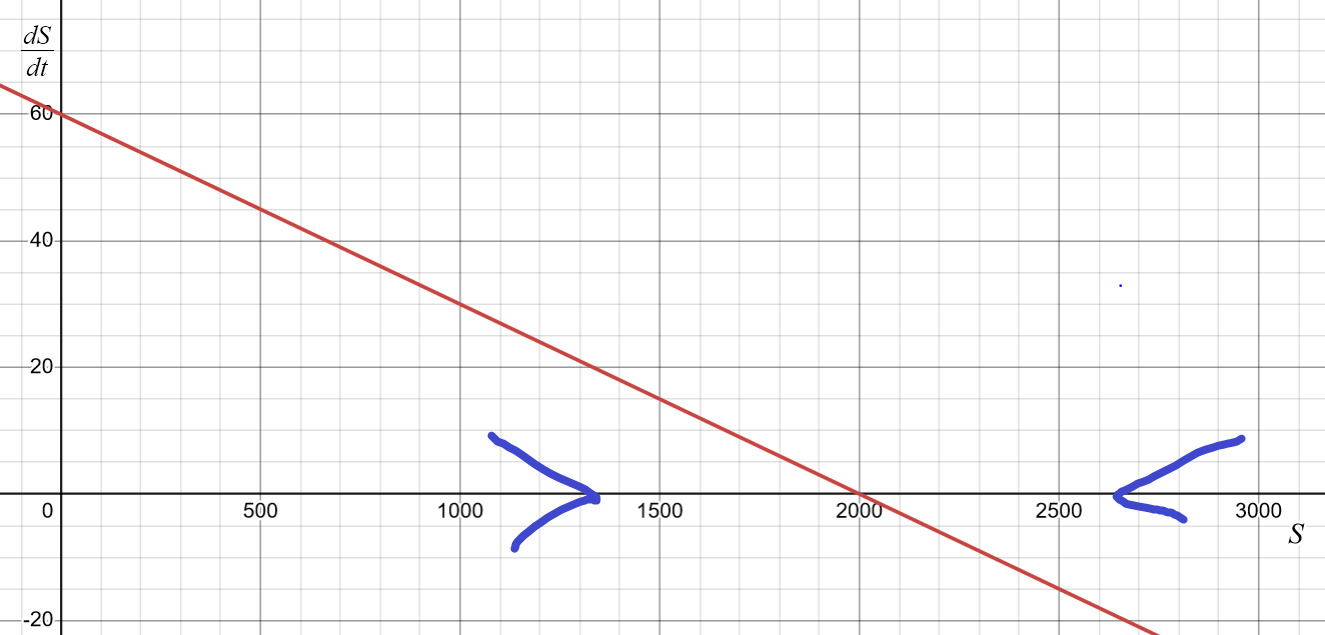
\includegraphics[width=0.49\textwidth]{images/7.5.9-phase-graph.png}
        \end{center}
    \end{multicols}
        
    \end{red}
    \item Suppose that there is initially no salt in the tank. Find the amount of salt $S(t)$ in minute $t$.

    \begin{red}
        Let's begin by separating and solving. I'm choosing to leave the $\frac{1}{100}$ on the right.
        \begin{align*}
            \dfrac{dS}{dt} &= \dfrac{1}{100}\left(6000 - 3S\right) \\
            \int \dfrac{1}{6000-3S} \ dS &= \int \dfrac{1}{100}\ dt \\
            -\dfrac{1}{3}\ln(6000 - 3S) &= \dfrac{1}{100}t + C \\
            \ln(6000 - 3S) &= -\dfrac{3}{100}t + C \\
            6000 - 3S &= C\cdot \exp\left(-\tfrac{3}{100}t\right) \\
            S(t) &= 2000 - C\cdot \exp\left(-\tfrac{3}{100}t\right) \\
            0 = S(0) &= 2000 - C\cdot \exp\left(-\tfrac{3}{100}\cdot 0\right) \\
            C &= 2000 \\
            S(t) &= 2000 - 2000\cdot \exp\left(-\tfrac{3}{100}t\right)
        \end{align*}
    \end{red}
    \item What happens to $S(t)$ after a very long time? Explain how you could have predicted this only knowing how much salt there is in each gallon of the briny solution that enters the tank.

    \begin{red}
        $S(t)$ rises toward the stable equilibrium of 2000 grams. This makes sense because the concentration of brine in the tank ($\tfrac{S(t)}{100}$ grams per gallon) will eventually match the concentration of brine flowing in (20 grams per gallon).
    \end{red}
\end{enumerate}

\end{enumerate}
\end{document}